\section{¿Por qué esta charla?}

\begin{frame}[t]{Una conversación real}
  \begin{itemize}
    \item Conversación con empresa líder en su sector.
      \begin{itemize}
        \item ¿Qué tipo de titulados buscas?
        \item Desarrolladores de C/C++.
        \item Últimamente parece que todo el mundo quiere ser desarrollador Java o gestor.
      \end{itemize}
    \item \pause Necesidades:
      \begin{itemize}
        \item Gestión dinámica de memoria.
        \item Gestión de recursos.
        \item Uso extendido de hilos y procesos.
        \item Herramientas de \emph{profiling} y depuración.
        \item Memoria compartida.
        \item Programación paralela.
      \end{itemize}
  \end{itemize}
\end{frame}

\begin{frame}[t]{En busca del lenguaje perfecto}
  \begin{columns}
    \begin{column}{0.3\textwidth}
      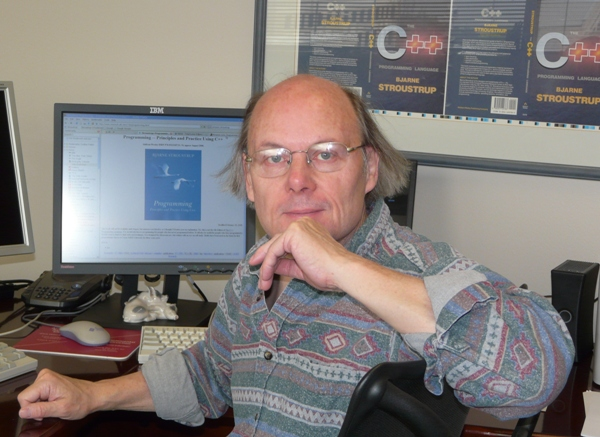
\includegraphics[width=\textwidth]{images/stroustrup.jpg}

      \emph{Bjarne Stroustrup}
    \end{column}
    \begin{column}{0.7\textwidth}
      \begin{quote}
        Anybody who comes to you and says he has a perfect language is either naive or a salesman.
      \end{quote}
      \pause
      \begin{quote}
        There are only two kinds of languages: the ones people complain about and the ones nobody uses.
      \end{quote}
      \pause
      \begin{quote}
        People who think they know everything really annoy those of us who know we don't.
      \end{quote}
    \end{column}
  \end{columns}
\end{frame}

\begin{frame}[t]{The Perils of Java Schools}
  \begin{itemize}[<+->]
    \item Don't get me wrong: there's nothing wrong with Java as an implementation language.
      \begin{itemize}
        \item There are lots of things wrong with it but those will have to wait for a different article.
      \end{itemize}
    \item The last decade a large number of otherwise perfectly good schools have gone 100\% Java
    \item {[Programming with pointers]}\ldots is still important for some of the most exciting programming jobs.
    \item Without understanding functional programming, you can't invent MapReduce, the algorithm that makes Google so massively scalable.
  \end{itemize}
  {\tiny
  \url{http://www.joelonsoftware.com/articles/ThePerilsofJavaSchools.html}}
\end{frame}
